%%%%%%%%%%%%%%%%%%%%%%%%%%%%%%%%%%%%%%%%%%%%%%%%%%%%%%%%%%%
\section{DAGs and PP}
%%%%%%%%%%%%%%%%%%%%%%%%%%%%%%%%%%%%%%%%%%%%%%%%%%%%%%%%%%%
%
%
\begin{frame}[t, negative]
	\subsectionpage
\end{frame}
%
%
\begin{frame}
	{DAGs and PP}
	%
	\begin{columns}
		%
		\begin{column}{0.5\textwidth}
			%
			\begin{itemize}
				%
				\item \textcolor{blue}{Directed acyclic graphs (DAGs)}, are a type of structural causal model (SCM) \cite{Pearl_2009, Cinelli_et_al_2021}
				%
				\item DAGs can be represented by a \textcolor{blue}{structural model}, and its associated \textcolor{blue}{causal diagram}\footnote{reproduced from \citet{Cinelli_et_al_2021}.}.
				%
				\item we put distributional assumptions to the structural model through \textcolor{blue}{probabilistic programming (PP)} \cite{Jaynes_2003}. \\
				{\small \alert{(more in part 3)} }
				%
			\end{itemize}
			%
		\end{column}
		%
		\begin{column}{0.5\textwidth}  
			%
			\begin{equ}
				%
				M = \left\{ \begin{aligned} 
					Z \leftarrow & \; f_{Z}(U_{z}) \\
					X \leftarrow & \; f_{X}(Z, U_{x}) \\
					Y \leftarrow & \; f_{Y}(X, Z, U_{y}) \\
					U \sim & \; P(\pmb{U})
				\end{aligned} \right
				%
				\caption*{(a) structural model}
				%
			\end{equ}
			%
			\begin{figure}
				%
				\begin{tikzpicture}
				% nodes
				\node[formula] at (-2,0) {$U_{X}$};
				\node[formula] at (-1,-0.3) {$X$};
				\node[formula] at (1,1.5) {$U_{Z}$};
				\node[formula] at (0,1) {$Z$};
				\node[formula] at (2,0) {$U_{Y}$};
				\node[formula] at (1,-0.3) {$Y$};
					
				% paths
				\draw [{Circle}-{latex}](-1.7,0)--(-1,0); % Ux->X
				\draw [{Circle}-{latex}](-1,0)--(0.9,0); % X->Y
				\draw [{Circle}-{latex}{Circle}](1.7,0)--(0.9,0); % Uy->Y
				\draw [{Circle}-{latex}](0.1,0.8)--(-0.9,0.1); % Z->X
				\draw [-{latex}](0.1,0.75)--(0.9,0.1); % Z->Y
				\draw [{Circle}-{latex}](0.9,1.3)--(0.1,0.8); % Uz->Z
				\end{tikzpicture}
				%
				\caption*{(b) causal diagram }
				%
			\end{figure}
			%
		\end{column}
		%
	\end{columns}
	%
\end{frame}
%
%
\begin{frame}
	{DAGs and PP}
	%
	\begin{columns}
		%
		\begin{column}{0.5\textwidth}
			%
			\begin{itemize}
				%
				\item $\pmb{V}=\{Z,X,Y\}$ are called \textcolor{blue}{endogenous variables}.
				%
				\item $\pmb{U}=\{U_{Z},U_{X},U_{Y}\}$ are called \textcolor{blue}{exogenous variables}. \\
				{\small \alert{(drawn when strictly required)} }
				%
				\item $\pmb{F}=\{f_{Z},f_{X},f_{Y}\}$ are called \textcolor{blue}{structural equations}.
				%
			\end{itemize}
			%
		\end{column}
		%
		\begin{column}{0.5\textwidth}  
			%
			\begin{equ}
				%
				M = \left\{ \begin{aligned} 
					Z \leftarrow & \; f_{Z}(U_{Z}) \\
					X \leftarrow & \; f_{X}(Z, U_{X}) \\
					Y \leftarrow & \; f_{Y}(X, Z, U_{Y}) \\
					U \sim & \; P(\pmb{U})
				\end{aligned} \right
				%
				\caption*{(a) structural model}
				%
			\end{equ}
			%
			\begin{figure}
				%
				\begin{tikzpicture}
					% nodes
					\node[formula] at (-2,0) {$U_{X}$};
					\node[formula] at (-1,-0.3) {$X$};
					\node[formula] at (1,1.5) {$U_{Z}$};
					\node[formula] at (0,1) {$Z$};
					\node[formula] at (2,0) {$U_{Y}$};
					\node[formula] at (1,-0.3) {$Y$};
					
					% paths
					\draw [{Circle}-{latex}](-1.7,0)--(-1,0); % Ux->X
					\draw [{Circle}-{latex}](-1,0)--(0.9,0); % X->Y
					\draw [{Circle}-{latex}{Circle}](1.7,0)--(0.9,0); % Uy->Y
					\draw [{Circle}-{latex}](0.1,0.8)--(-0.9,0.1); % Z->X
					\draw [-{latex}](0.1,0.75)--(0.9,0.1); % Z->Y
					\draw [{Circle}-{latex}](0.9,1.3)--(0.1,0.8); % Uz->Z
				\end{tikzpicture}
				%
				\caption*{(b) causal diagram }
				%
			\end{figure}
			%
		\end{column}
		%
	\end{columns}
	%
\end{frame}
%
%
\begin{frame}
	{DAGs and PP}
	%
	\begin{columns}
		%
		\begin{column}{0.5\textwidth}
			%
			Causal diagram conventions \cite{Cinelli_et_al_2021},
			%
			\begin{itemize}
				%
				\item \colorbox{gray}{black nodes} are \textcolor{blue}{observed variables}.
				%
				\item \colorbox{grey}{\textcolor{gray}{white nodes}} are \textcolor{blue}{unobserved variables}.
				%
				\item \colorbox{gray}{\alert{red nodes}} are variables for which we will decide its inclusion or not.
				%
			\end{itemize}
			%
		\end{column}
		%
		\begin{column}{0.5\textwidth}  
			%
			\begin{equ}
				%
				M = \left\{ \begin{aligned} 
					Z \leftarrow & \; f_{Z}(U_{Z}) \\
					X \leftarrow & \; f_{X}(Z, U_{X}) \\
					Y \leftarrow & \; f_{Y}(X, Z, U_{Y}) \\
					U \sim & \; P(\pmb{U})
				\end{aligned} \right
				%
				\caption*{(a) structural model}
				%
			\end{equ}
			%
			\begin{figure}
				%
				\begin{tikzpicture}
					% nodes
					\node[formula] at (-2,0) {$U_{X}$};
					\node[formula] at (-1,-0.3) {$X$};
					\node[formula] at (1,1.5) {$U_{Z}$};
					\node[formula] at (0,1) {$Z$};
					\node[formula] at (2,0) {$U_{Y}$};
					\node[formula] at (1,-0.3) {$Y$};
					
					% paths
					\draw [{Circle [open]}-{latex}{Circle}](-1.7,0)--(-0.9,0); % Ux->X
					\draw [-{latex}](-0.9,0)--(0.9,0); % X->Y
					\draw [{Circle [open]}-{latex}{Circle}](1.7,0)--(0.9,0); % Uy->Y
					\draw [{Circle [color=red]}-{latex}](0.1,0.8)--(-0.9,0.1); % Z->X
					\draw [-{latex}](0.1,0.75)--(0.9,0.1); % Z->Y
					\draw [{Circle [open]}-{latex}](0.9,1.3)--(0.1,0.8); % Uz->Z
				\end{tikzpicture}
				%
				\caption*{(b) causal diagram }
				%
			\end{figure}
			%
		\end{column}
		%
	\end{columns}
	%
\end{frame}
%
%
\begin{frame}
	{DAGs and PP}
	%
	\begin{columns}
		%
		\begin{column}{0.5\textwidth}
			%
			Other causal diagram conventions,
			%
			\begin{itemize}
				%
				\item \colorbox{gray}{no circle} nodes are \textcolor{blue}{observed variables}.
				%
				\item \colorbox{gray}{circled} nodes are \textcolor{blue}{unobserved variables}.
				%
				\item \colorbox{gray}{squared} nodes are variables for which we will decide its inclusion or not.
				%
			\end{itemize}
			%
		\end{column}
		%
		\begin{column}{0.5\textwidth}  
			%
			\begin{equ}
				%
				M = \left\{ \begin{aligned} 
					Z \leftarrow & \; f_{Z}(U_{Z}) \\
					X \leftarrow & \; f_{X}(Z, U_{X}) \\
					Y \leftarrow & \; f_{Y}(X, Z, U_{Y}) \\
					U \sim & \; P(\pmb{U})
				\end{aligned} \right
				%
				\caption*{(a) structural model}
				%
			\end{equ}
			%
			\begin{figure}
				%
				\begin{tikzpicture}
					% nodes
					\node[formula, draw, circle] at (-2.5,0) {$U_{X}$};
					\node[formula] at (-1,0) {$X$};
					\node[formula, draw, circle] at (1.5,1.5) {$U_{Z}$};
					\node[formula, draw, rectangle] at (0,1) {$Z$};
					\node[formula, draw, circle] at (2.5,0) {$U_{Y}$};
					\node[formula] at (1,0) {$Y$};
					
					% paths
					\draw [-{latex}](-2,0)--(-1.2,0); % Ux->X
					\draw [-{latex}](-0.8,0)--(0.8,0); % X->Y
					\draw [-{latex}](2,0)--(1.2,0); % Uy->Y
					\draw [-{latex}](0,0.7)--(-0.8,0.2); % Z->X
					\draw [-{latex}](0,0.7)--(0.8,0.2); % Z->Y
					\draw [-{latex}](1,1.3)--(0.3,1); % Uz->Z
				\end{tikzpicture}
				%
				\caption*{(b) causal diagram }
				%
			\end{figure}
			%
		\end{column}
		%
	\end{columns}
	%
\end{frame}
%
%
\begin{frame}
	{The benign case of DAG elementals}
	{For everything can be depicted with them}
	%
	\begin{columns}
		%
		\begin{column}{0.3\textwidth}
			%
			\begin{figure}
				%
				\begin{tikzpicture}
					% nodes
					\node[formula] at (-1,0.5) {$Z$};
					\node[formula] at (1,1) {$X$};
					\node[formula] at (1,0) {$Y$};
					
					% paths
					\draw [{Circle}-{latex}{Circle}](-0.85,0.5)--(0.8,1); % Z->X
					\draw [-{latex}{Circle}](-0.85,0.55)--(0.8,0); % Z->Y
				\end{tikzpicture}
				%
				\caption*{(a) fork}
				%
			\end{figure}
			%
			\begin{figure}
				%
				\begin{tikzpicture}
					% nodes
					\node[formula] at (-2,0.5) {$D$};
					\node[formula] at (-0.55,0.2) {$Z$};
					\node[formula] at (1,1) {$X$};
					\node[formula] at (1,0) {$Y$};
					
					% paths
					\draw [{Circle}-{latex}{Circle}](-0.5,0.5)--(-1.8,0.5); % Z->D
					\draw [-{latex}{Circle}](-0.5,0.55)--(0.8,1); % Z->X
					\draw [-{latex}{Circle}](-0.5,0.45)--(0.8,0); % Z->Y
				\end{tikzpicture}
				%
				\caption*{(d) descendant on fork}
				%
			\end{figure}
			%
		\end{column}
		%
		%
		\begin{column}{0.3\textwidth}
			%
			\begin{figure}
				%
				\begin{tikzpicture}
					% nodes
					\node[formula] at (-1,0) {$X$};
					\node[formula] at (0.05,0) {$Z$};
					\node[formula] at (1,0) {$Y$};
					
					% paths
					\draw [{Circle}-{latex}](-1,0.3)--(0,0.3); % X->Z
					\draw [{Circle}-{latex}{Circle}](0,0.3)--(1,0.3); % Z->Y
				\end{tikzpicture}
				%
				\caption*{(b) pipe}
				%
			\end{figure}
			%
			\begin{figure}
				%
				\begin{tikzpicture}
					% nodes
					\node[formula] at (-1,0) {$X$};
					\node[formula] at (0.1,1.5) {$D$};
					\node[formula] at (0.05,0) {$Z$};
					\node[formula] at (1,0) {$Y$};
					
					% paths
					\draw [{Circle}-{latex}](-1,0.3)--(0,0.3); % X->Z
					\draw [{Circle}-{latex}{Circle}](0,0.3)--(1,0.3); % Z->Y
					\draw [-{latex}{Circle}](0.05,0.3)--(0.05,1.3); % Z->D
				\end{tikzpicture}
				%
				\caption*{(e) descendant on pipe}
				%
			\end{figure}
			%
		\end{column}
		%
		%
		\begin{column}{0.3\textwidth}  
			%
			\begin{figure}
				\begin{tikzpicture}
					% nodes
					\node[formula] at (-1,1) {$X$};
					\node[formula] at (-1,0) {$Y$};
					\node[formula] at (1,0.5) {$Z$};
					
					% paths
					\draw [{Circle}-{latex}{Circle}](-0.8,0.9)--(0.8,0.5); % X->Z
					\draw [{Circle}-{latex}](-0.8,0.1)--(0.68,0.5); % Y->Z
				\end{tikzpicture}
				%
				\caption*{(c) collider}
				%
			\end{figure}
			%
			\begin{figure}
				%
				\begin{tikzpicture}
					% nodes
					\node[formula] at (-1,1) {$X$};
					\node[formula] at (-1,0) {$Y$};
					\node[formula] at (0.55,0.2) {$Z$};
					\node[formula] at (2,0.5) {$D$};
					
					% paths
					\draw [{Circle}-{latex}](-0.8,0.9)--(0.5,0.55); % X->Z
					\draw [{Circle}-{latex}](-0.8,0.1)--(0.5,0.45); % Y->Z
					\draw [{Circle}-{latex}{Circle}](0.5,0.5)--(1.8,0.5); % Z->D
				\end{tikzpicture}
				%
				\caption*{(f) descendant on collider}
				%
			\end{figure}
			%
		\end{column}
		%
	\end{columns}
	%
\end{frame}
%
%
\begin{frame}
	{About D-separation}
	%
	\begin{columns}
		%
		\begin{column}{0.5\textwidth}
			%
			Causal graph theory \cite{Pearl_1988, Pearl_2009, Pearl_et_al_2016, Pearl_et_al_2018, Spirtes_et_al_1991},
			%
			\begin{enumerate}
				%
				\item \textcolor{blue}{descendant} (child, grandchild), \textcolor{blue}{parent} (grandparent). \\
				{\small \alert{(path specific)} }
				%
				\item paths (\textcolor{blue}{directional}, \textcolor{blue}{non-directional}).
				%
				\item paths are \textcolor{blue}{blocked} or \textcolor{blue}{open} according to the \textcolor{blue}{D-separation} rules. \\
				{\small \alert{(also path specific)} }
				%
				\item there are only \textcolor{blue}{four (4)} D-separation rules.
				%
			\end{enumerate}
			%
		\end{column}
		%
		\begin{column}{0.5\textwidth}  
			%
			\begin{equ}
				%
				M = \left\{ \begin{aligned} 
					Z \leftarrow & \; f_{Z}(U_{Z}) \\
					X \leftarrow & \; f_{X}(Z, U_{X}) \\
					Y \leftarrow & \; f_{Y}(X, Z, U_{Y}) \\
					U \sim & \; P(\pmb{U})
				\end{aligned} \right
				%
				\caption*{(a) structural model}
				%
			\end{equ}
			%
			\begin{figure}
				%
				\begin{tikzpicture}
					% nodes
					\node[formula] at (-2,0) {$U_{X}$};
					\node[formula] at (-1,-0.3) {$X$};
					\node[formula] at (1,1.5) {$U_{Z}$};
					\node[formula] at (0,1) {$Z$};
					\node[formula] at (2,0) {$U_{Y}$};
					\node[formula] at (1,-0.3) {$Y$};
					
					% paths
					\draw [{Circle [open]}-{latex}](-1.7,0)--(-1,0); % Ux->X
					\draw [{Circle}-{latex}](-1,0)--(0.9,0); % X->Y
					\draw [{Circle [open]}-{latex}{Circle}](1.7,0)--(0.9,0); % Uy->Y
					\draw [{Circle [color=red]}-{latex}](0.1,0.8)--(-0.9,0.1); % Z->X
					\draw [-{latex}](0.1,0.75)--(0.9,0.1); % Z->Y
					\draw [{Circle [open]}-{latex}](0.9,1.3)--(0.1,0.8); % Uz->Z
				\end{tikzpicture}
				%
				\caption*{(b) causal diagram}
				%
			\end{figure}
			%
		\end{column}
		%
	\end{columns}
	%
\end{frame}
%
%
\begin{frame}
	{About D-separation}
	%
	\begin{columns}
		%
		\begin{column}{0.5\textwidth}
			%
			The D-separation (Directional) rules \cite{Hernan_2020},
			%
			\begin{enumerate}
				%
				\item If no variables being conditioned on, a path is blocked if and only if, two arrowheads on the path collide at some variable on the path.
				%
				\item Any path that contains a noncollider that has been conditioned on, is blocked \textcolor{blue}{(backdoor path)}\footnote{there is also a \textcolor{blue}{front-door path} (if you wonder).}.
				%
				\item A collider that has been conditioned on does not block a path.
				%
				\item A collider that has a descendant that has been conditioned on does not block a path.
				%
			\end{enumerate}
			%
		\end{column}
		%
		\begin{column}{0.5\textwidth}  
			%
			\begin{figure}
				%
				\begin{tikzpicture}
					% nodes
					\node[formula] at (-1,1) {$X$};
					\node[formula] at (-1,0) {$Y$};
					\node[formula] at (1,0.5) {$Z$};
					
					% paths
					\draw [{Circle}-{latex}{Circle}](-0.8,0.9)--(0.8,0.5); % X->Z
					\draw [{Circle}-{latex}](-0.8,0.1)--(0.69,0.5); % Y->Z
				\end{tikzpicture}
				%
			\end{figure}
			%
			\begin{figure}
				%
				\begin{tikzpicture}
					% nodes
					\node[formula] at (-1,0.5) {$Z$};
					\node[formula] at (1,1) {$X$};
					\node[formula] at (1,0) {$Y$};
					
					% paths
					\draw [{Circle [color=red]}-{latex}{Circle}](-0.85,0.5)--(0.8,1); % Z->X
					\draw [-{latex}{Circle}](-0.75,0.50)--(0.8,0); % Z->Y
				\end{tikzpicture}
				%
			\end{figure}
			%
			\begin{figure}
				%
				\begin{tikzpicture}
					% nodes
					\node[formula] at (-1,0) {$X$};
					\node[formula] at (0,0) {$Z$};
					\node[formula] at (1,0) {$Y$};
					
					% paths
					\draw [{Circle}-{latex}](-1,0.3)--(0,0.3); % X->Z
					\draw [{Circle [color=red]}-{latex}{Circle}](0,0.3)--(1,0.3); % Z->Y
				\end{tikzpicture}
				%
			\end{figure}
			%
			\begin{figure}
				%
				\begin{tikzpicture}
					% nodes
					\node[formula] at (-1,1) {$X$};
					\node[formula] at (-1,0) {$Y$};
					\node[formula] at (0.55,0.2) {$Z$};
					\node[formula] at (2,0.5) {$D$};
					
					% paths
					\draw [{Circle}-{latex}](-0.8,0.9)--(0.49,0.55); % X->Z
					\draw [{Circle}-{latex}](-0.8,0.1)--(0.49,0.45); % Y->Z
					\draw [{Circle [color=red]}-{latex [color=red]}](0.5,0.5)--(1.8,0.5); % Z->D
				\end{tikzpicture}
				%
			\end{figure}
			%
		\end{column}
		%
	\end{columns}
	%
\end{frame}
%
%
\begin{frame}
	{About D-separation}
	%
	\begin{columns}
		%
		\begin{column}{0.5\textwidth}
			%
			The D-separation rules \textcolor{blue}{implications}, \\			{\small (independent of distributional assumptions)}
			%
			\begin{enumerate}
				%
				\item $\dsep{X}{Y} \; \Longrightarrow \;$ \\
				$P(X,Y) = P(X) \cdot P(Y)$
				%
				\item $\dsep{X}{Y} \; | \; Z \Longrightarrow \;$ \\
				$P(X,Y|Z) = P(X|Z) \cdot P(Y|Z)$ \\
				{\small \alert{(same for fork or pipe)} }
				%
				\item $\ndsep{X}{Y} \; | \; Z \Longrightarrow \;$ \\
				$P(X,Y|Z) \neq P(X|Z) \cdot P(Y|Z)$ 
				%
				\item $\ndsep{X}{Y} \; | \; D \Longrightarrow \;$ \\
				$P(X,Y|D) \neq P(X|D) \cdot P(Y|D)$
				%
			\end{enumerate}
			%
		\end{column}
		%
		\begin{column}{0.5\textwidth}  
			%
			\begin{figure}
				%
				\begin{tikzpicture}
					% nodes
					\node[formula] at (-1,1) {$X$};
					\node[formula] at (-1,0) {$Y$};
					\node[formula] at (1,0.5) {$Z$};
					
					% paths
					\draw [{Circle}-{latex}{Circle}](-0.8,0.9)--(0.8,0.5); % X->Z
					\draw [{Circle}-{latex}](-0.8,0.1)--(0.69,0.5); % Y->Z
				\end{tikzpicture}
				%
			\end{figure}
			%
			\begin{figure}
				%
				\begin{tikzpicture}
					% nodes
					\node[formula] at (-1,0.5) {$Z$};
					\node[formula] at (1,1) {$X$};
					\node[formula] at (1,0) {$Y$};
					
					% paths
					\draw [{Circle [color=red]}-{latex}{Circle}](-0.85,0.5)--(0.8,1); % Z->X
					\draw [-{latex}{Circle}](-0.85,0.55)--(0.8,0); % Z->Y
				\end{tikzpicture}
				%
			\end{figure}
			%
			\begin{figure}
				%
				\begin{tikzpicture}
					% nodes
					\node[formula] at (-1,0) {$X$};
					\node[formula] at (0,0) {$Z$};
					\node[formula] at (1,0) {$Y$};
					
					% paths
					\draw [{Circle}-{latex}](-1,0.3)--(0,0.3); % X->Z
					\draw [{Circle [color=red]}-{latex}{Circle}](0,0.3)--(1,0.3); % Z->Y
				\end{tikzpicture}
				%
			\end{figure}
			%
			\begin{figure}
				%
				\begin{tikzpicture}
					% nodes
					\node[formula] at (-1,1) {$X$};
					\node[formula] at (-1,0) {$Y$};
					\node[formula] at (0.55,0.2) {$Z$};
					\node[formula] at (2,0.5) {$D$};
					
					% paths
					\draw [{Circle}-{latex}](-0.8,0.9)--(0.49,0.55); % X->Z
					\draw [{Circle}-{latex}](-0.8,0.1)--(0.49,0.45); % Y->Z
					\draw [{Circle [color=red]}-{latex [color=red]}](0.5,0.5)--(1.8,0.5); % Z->D
				\end{tikzpicture}
				%
			\end{figure}
			%
		\end{column}
		%
	\end{columns}
	%
\end{frame}
%
%
\begin{lhframe}[rhgraphic={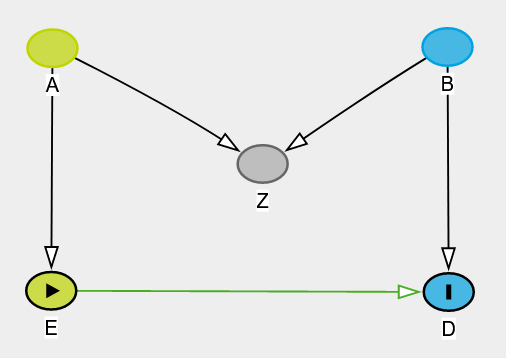
\includegraphics[scale=0.6]{DAGitty.png}}]
	{Oh DAGitty!! mijn vriendin}
	
	\begin{itemize}
		%
		\item browser (R package) environment for creating, editing, and analyzing causal diagrams \cite{Textor_et_al_2016}.
		%
		\item available online: \textcolor{blue}{\url{http://dagitty.net}}
		%
		\item But there are more fish in the sea: \textcolor{blue}{\url{http://www.causalfusion.net}} \cite{Bareinboim_et_al_2016} \\
		{\small (b**** better have my \$\$\$)}
		%
	\end{itemize}
	%
\end{lhframe}
%
%
\begin{lhframe}[rhgraphic={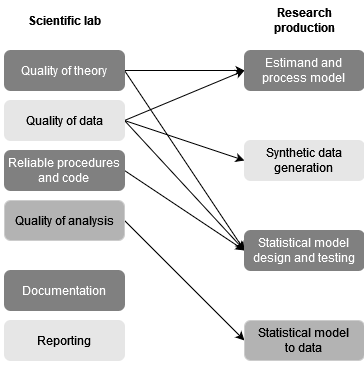
\includegraphics[scale=0.60]{DAG_to_research.png}}]
	{Where do DAGs and PP fit?}
	%
	\heading{starts with:}
	\begin{itemize}
		%
		\item A clear definition of the estimand and process model (assumptions).
		%
		\item An improved the reliability of your procedures.
		%
		\item As a documentation procedure.
		%
	\end{itemize}
	%
	\heading{and leads to:}
	\begin{itemize}
		%
		\item A sound analysis, and result \\
		{\small \alert{(even when we cannot have an answer to our question)} }
		%
		\item An improved planning to get data.
		%
	\end{itemize}
	%
\end{lhframe}
%
%